\documentclass[11pt]{article}
\usepackage[utf8]{inputenc}
\usepackage[T1]{fontenc}
\usepackage{amsmath}
\usepackage{amsfonts}
\usepackage{amssymb}
\usepackage[version=4]{mhchem}
\usepackage{stmaryrd}
\usepackage{graphicx}
\usepackage[export]{adjustbox}
\graphicspath{ {./images/} }

\begin{document}
Relative Value Multistrategy Funds

Relative value multistrategy (RVMS) funds simply combine one or more relative value strategies within a single fund. Rather than focusing on a single relative value strategy, such as convertible arbitrage, volatility arbitrage, or fixed-income arbitrage, managers diversify positions across these strategy types. The category of multistrategy relative value funds is extremely large.

\section*{Rationale of Relative Value Multistrategy Funds}
What is the rationale for building a RVMS fund rather than a single-strategy relative value fund? First, we know that some of the largest funds in the hedge fund universe are RVMS funds. Funds focusing on a smaller market may have capacity issues, finding that their assets have grown too large to effectively invest exclusively in one strategy, such as convertible arbitrage. Second, opportunities may be cyclical. If a manager believes that asset-backed securities currently offer a lower-risk or higher return investment than corporate debt arbitrage, allocations to the more attractive investment sector can be opportunistically increased. Finally, there is an opportunity for diversification. By investing across sectors, a multistrategy fund may be able to offer cost-effective access to diversification.

\section*{Key Observations Regarding Historical Returns of Relative Multistrategy Funds}
Monthly returns to relative value multistrategy funds are observed from January of 2000 to December of 2021, for a total of 264 observations. Statistical Summary of Returns provides univariate return statistics and partial autocorrelations of returns in the top panel, and a histogram of returns in the bottom panel.

\begin{center}
\begin{tabular}{lcc}
\hline
Index (Jan. 2000-Dec. 2021) & \begin{tabular}{c}
HFRI Relative Value: \\
Multi-Strategy Index \\
\end{tabular} & \begin{tabular}{c}
MSCI World \\
Equity \\
\end{tabular} \\
\hline
Annualized Arithmetic Mean & $5.2 \%$ & $6.8 \%$ \\
Annualized Standard Deviation & $4.3 \%$ & $15.4 \%$ \\
Annualized Semivolatility & $4.4 \%$ & $11.8 \%$ \\
Annualized Median & $6.5 \%$ & $15.1 \%$ \\
Skewness & -2.6 & -0.6 \\
Excess Kurtosis & 16.2 & 1.6 \\
Sharpe Ratio & 0.6 & 0.3 \\
Sortino Ratio & 0.6 & 0.4 \\
Annualized Geometric mean & $5.1 \%$ & $5.6 \%$ \\
First-Order Autocorrelation & 0.4 & 0.1 \\
Annualized Standard Deviation & $6.5 \%$ & $17.0 \%$ \\
(Adjusted for Autocorrelation) & $3.9 \%$ & $12.8 \%$ \\
Maximum & $-8.4 \%$ & $-19.0 \%$ \\
Minimum & $-21.5 \%$ & $-54.0 \%$ \\
Max Drawdown &  &  \\
\end{tabular}
\end{center}

\begin{center}
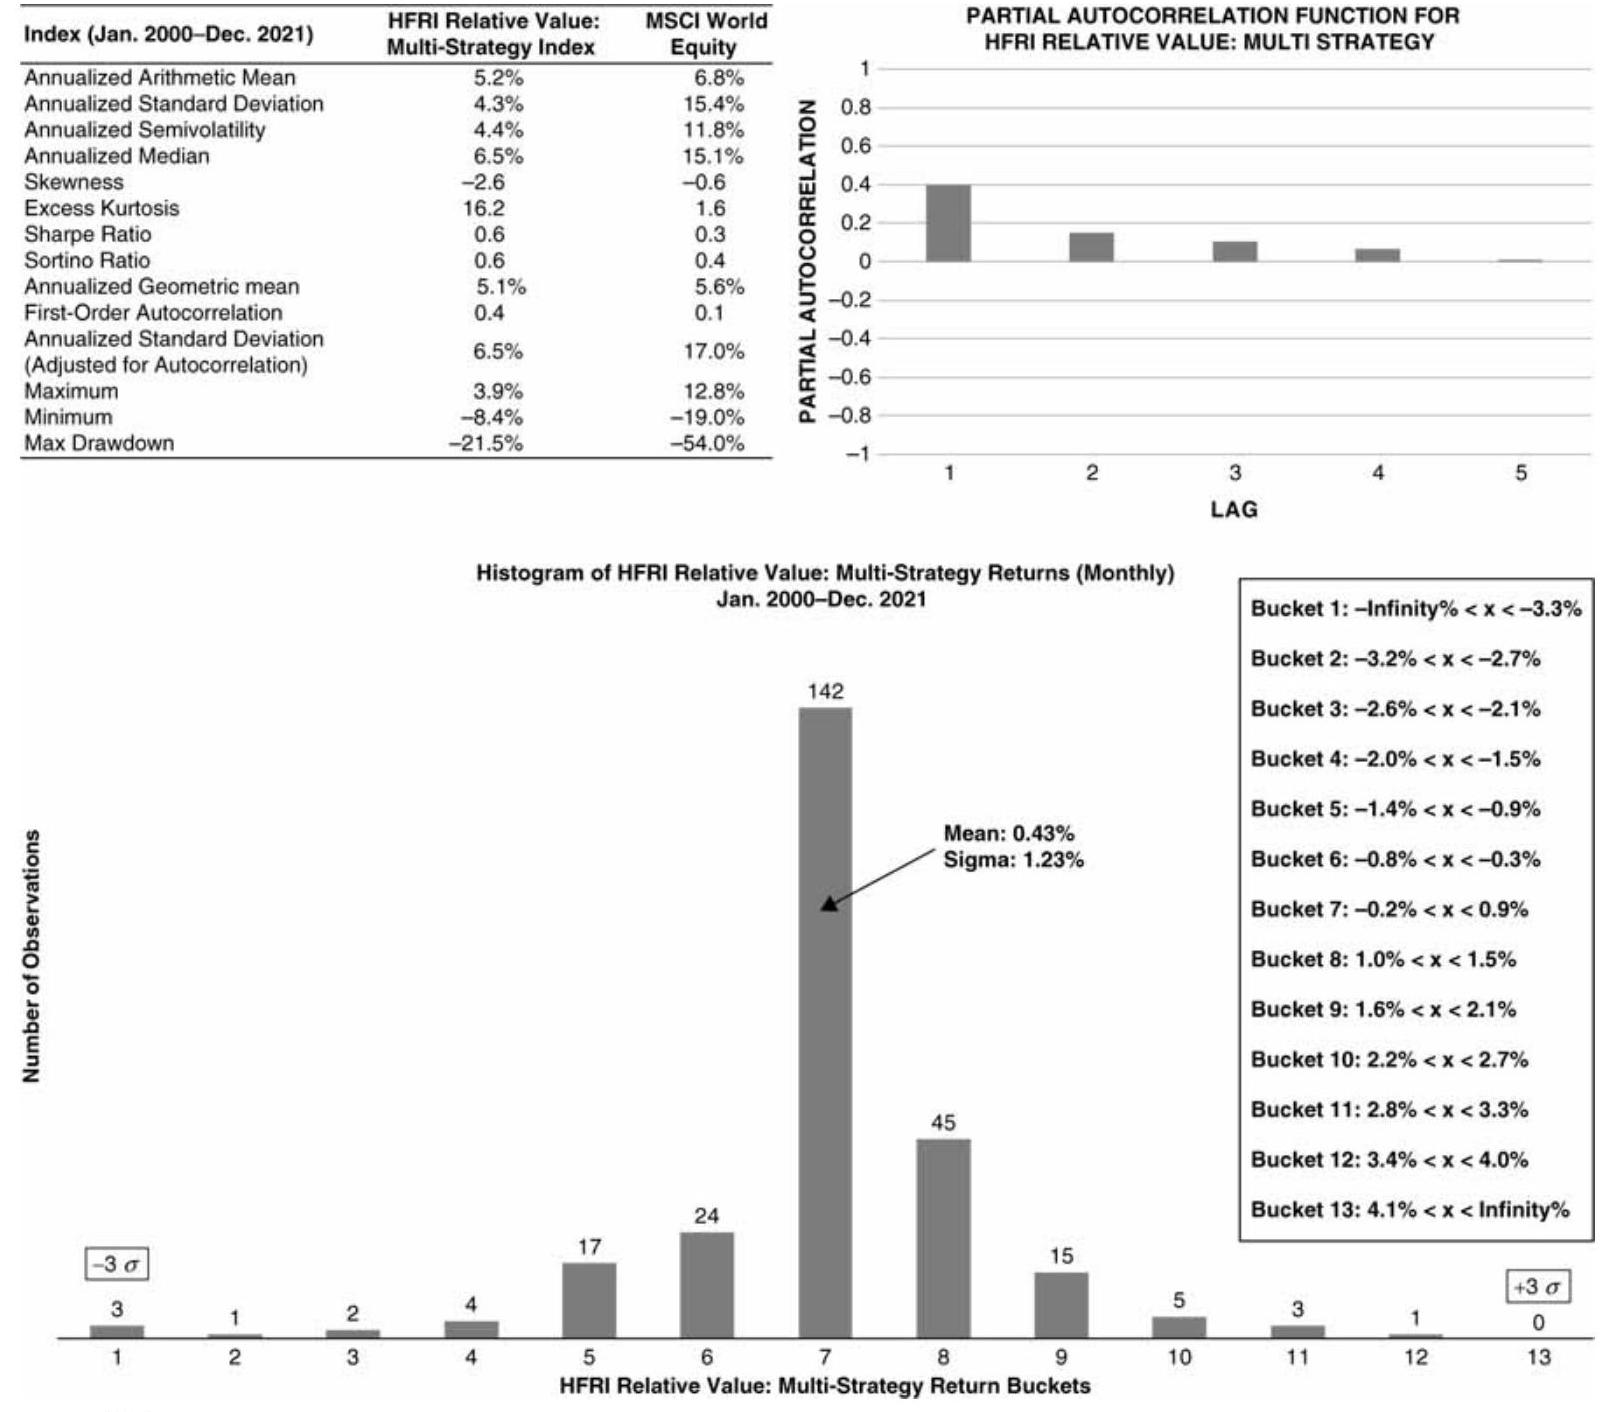
\includegraphics[max width=\textwidth]{2024_04_09_2019938a8e6abee55fc6g-2}
\end{center}

\section*{Statistical Summary of Returns}
Key observations on relative value multistrategy returns that are consistent with economic reasoning are an essential component of knowledge and include the following.

\begin{enumerate}
  \item The historic return distribution of HFRI Multi-Strategy exhibited moderately greater left skew and very high excess kurtosis relative to global equities.

  \item Volatility of returns was very substantially lower than that of world equities.

  \item Returns exhibited strong positive first-order autocorrelation.

  \item Maximum drawdown was moderately milder than observed for global equities.

\end{enumerate}

In conclusion, we note similar observations regarding the returns across all relative value strategies. These strategies tend to invest in fixed-income securities, some of which are less liquid, which is noted by the strong autocorrelation of returns. These strategies also tend to have extreme levels of negative skewness and excess kurtosis, because the large losses during liquidity crisis events are out of character with the smooth positive returns experienced in normal markets.


\end{document}